\documentclass[14pt]{article}
\usepackage{graphicx}
\usepackage[left=3cm, right=1.5cm, top=1.5cm, bottom=2cm]{geometry}
\usepackage[russian]{babel}
\usepackage[T2A]{fontenc}
\usepackage[utf8]{inputenc}
\usepackage[unicode]{hyperref}
\usepackage{a4wide}
\usepackage{pdfpages}

\begin{document}

\includepdf[pages=-]{title_Ali.pdf}
\clearpage
\tableofcontents
\clearpage
\section{Команда}
\section{Ресурсы}
	\subsection{Сетевой график}
	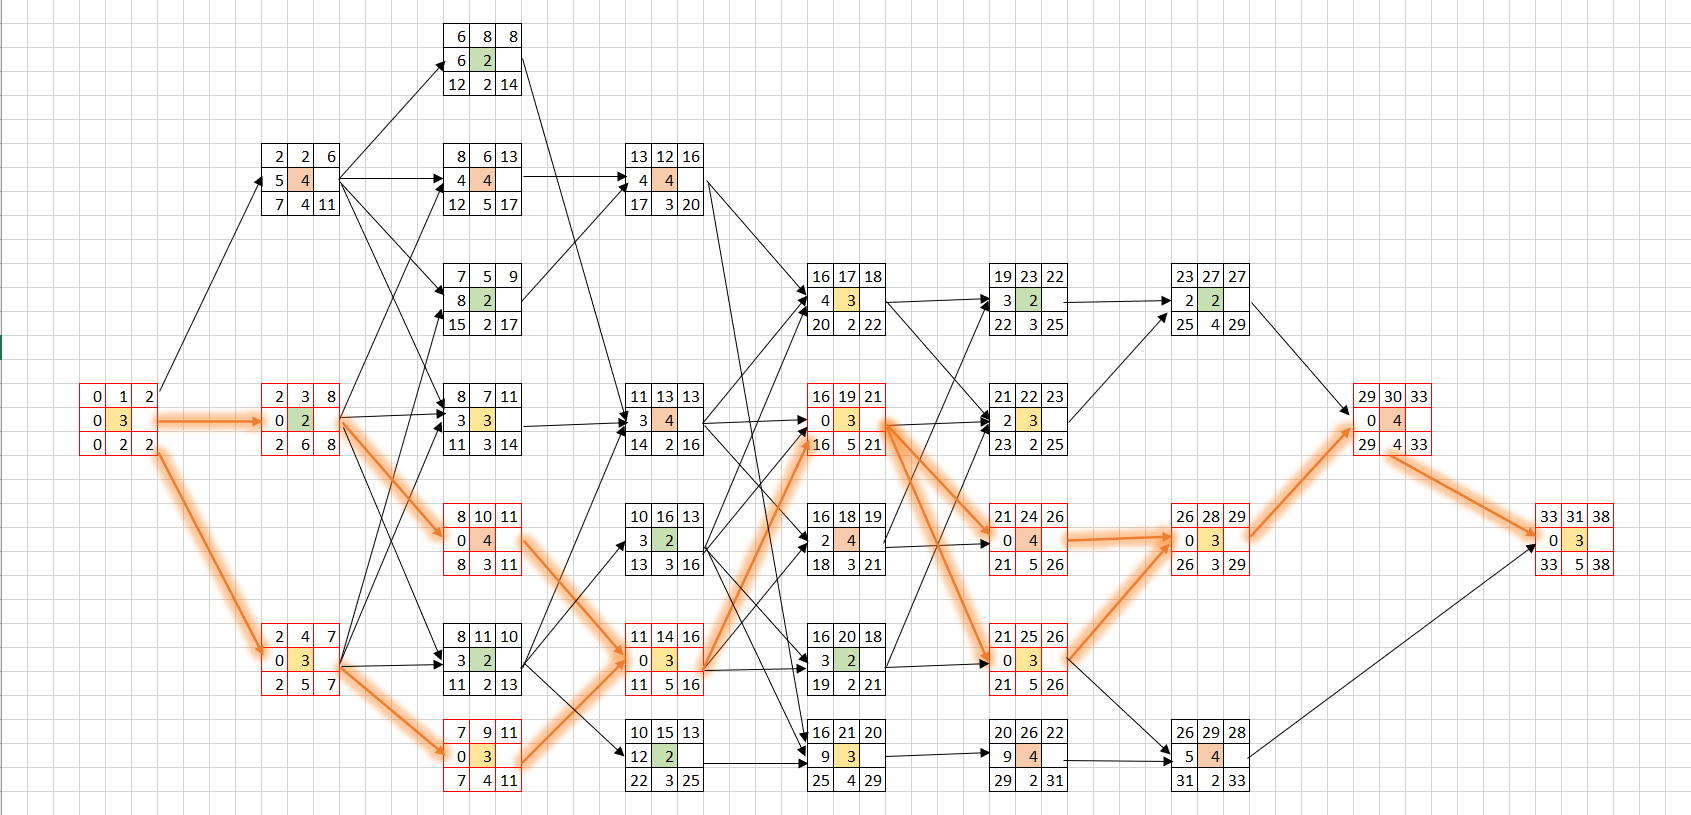
\includegraphics[width=\textwidth]{../img/init_network_graph.png}\\
	В проекте 4 попарно различных кретических пути.
	\subsection{Назначение ресурсов}
	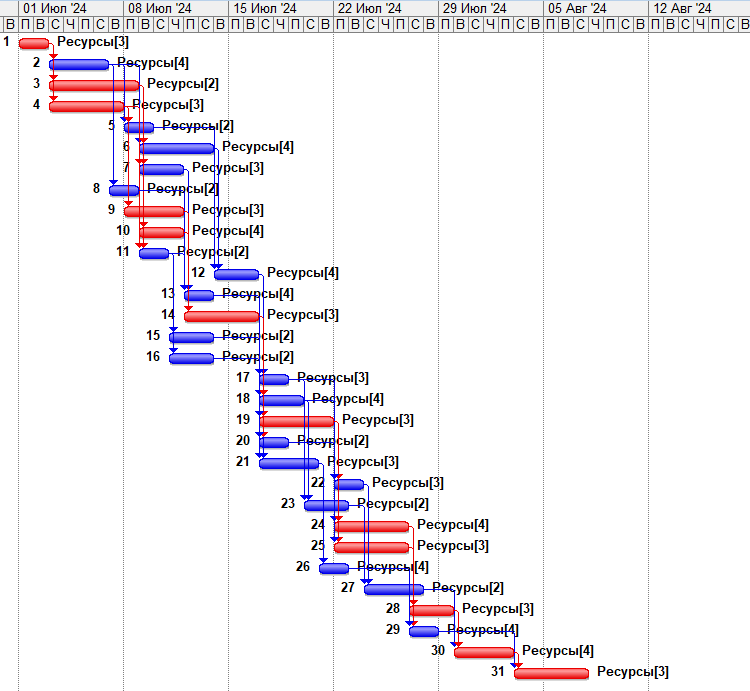
\includegraphics[width=\textwidth]{../img/init_resource_manage.png}
\section{Задача}
	Попробовать уменьшить количество используемых ресурсов до 5 в день,
		меняя при этом длительность работ не более чем на 2 дня.
	Дата окончания проекта может меняться.
\section{Решение}
	Раз можно менять дату окончания проекта, то можно без всяких изменений продолжительностей работ передвинуть все задачи.
	Чтобы не было такого грубого решения предлагаю ограничить время выполнения проекта двумя месяцами.
	\subsection{Первый вариант}
		Свобода в дате окончания проекта позволила обойтись минимальными изменениями.
		Обращаю внимание на то, что проект заканчивается \texttt{30.08}!\\
		{\LARGE Что поменяли:}\\
		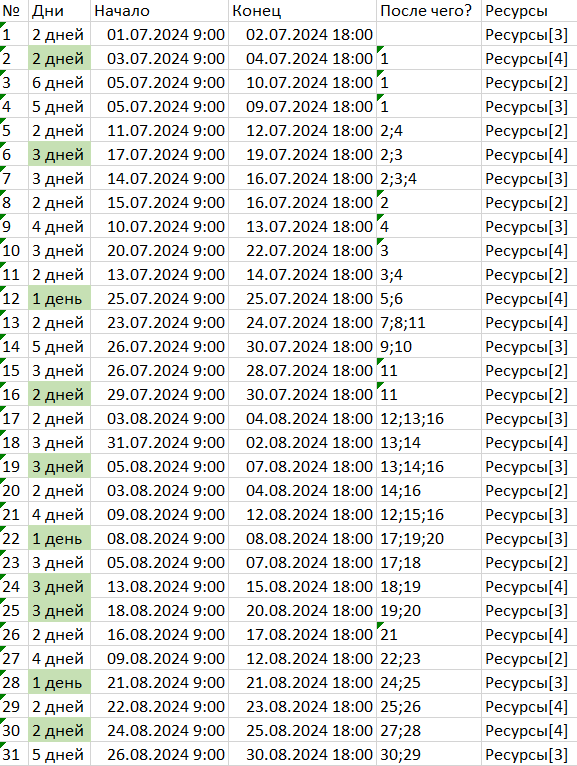
\includegraphics[height=0.6\textheight]{../img/2a1_days_change.png}\\ 
		{\LARGE Как это выглядит:}\\
		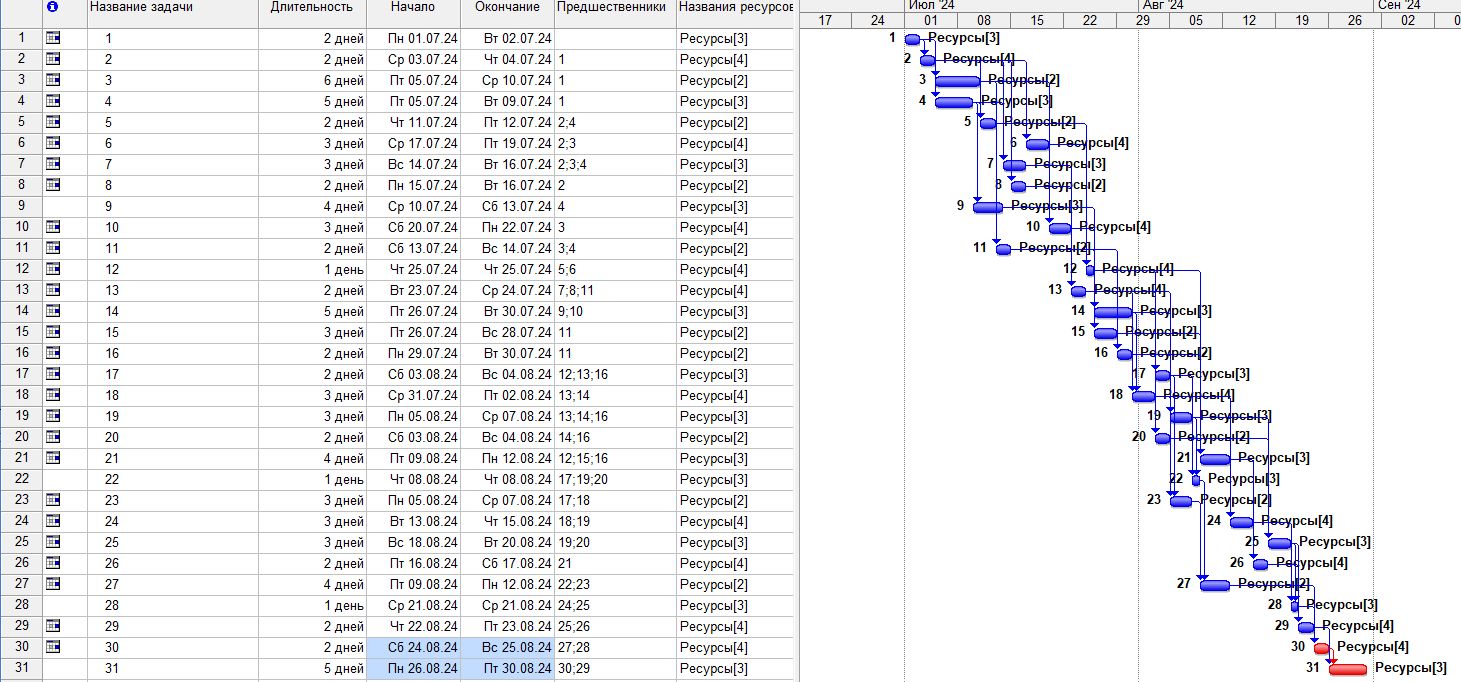
\includegraphics[width=\textwidth]{../img/ot2a1_1.png}\\
		Обращаю внимание, что <<Четвёрки>> (см отчёт первого задания) не могут идти параллельно любой другой задачк,
			поэтому их продолжительность сокращать очень выгодно.\\
		{\LARGE Cколько оно тратит:}\\
		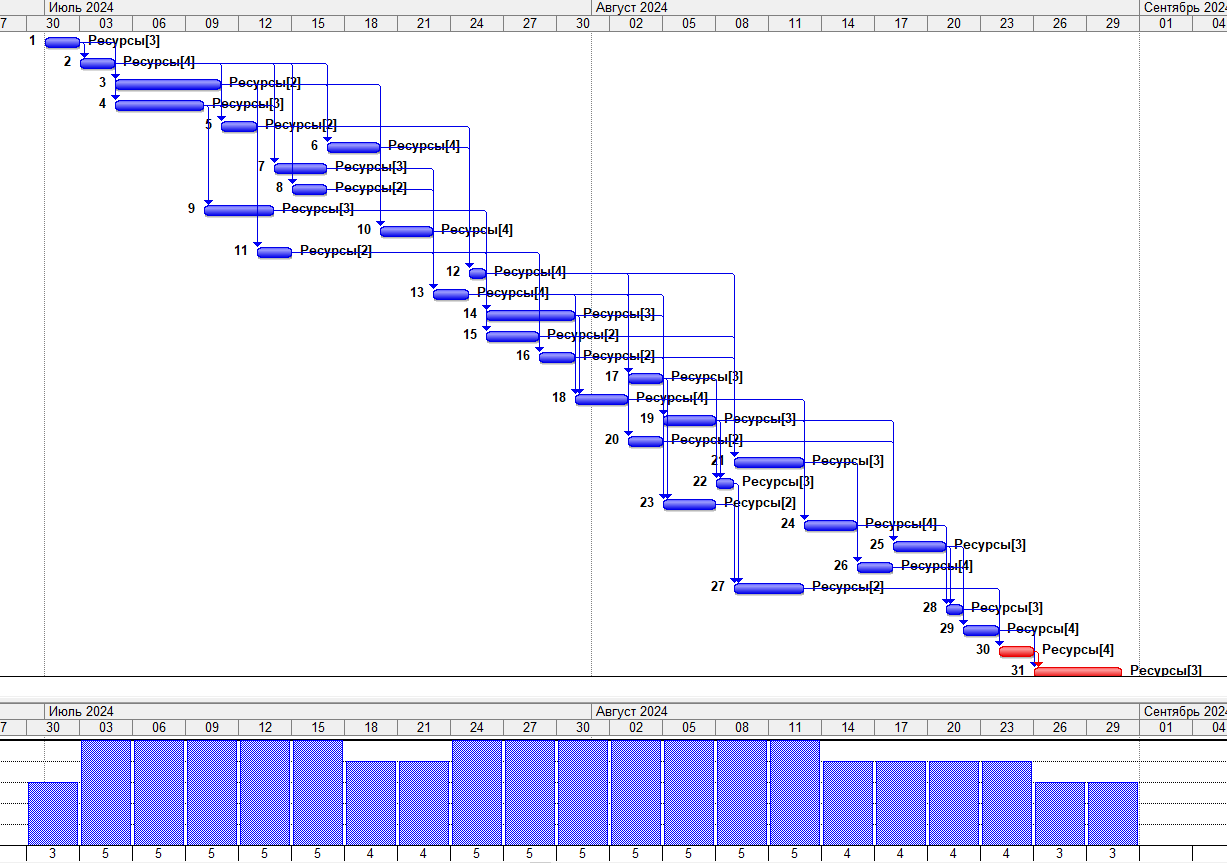
\includegraphics[width=\textwidth]{../img/2a1_answer.png}\\ 
	\subsection{Второй вариант}
		Теперь попробуем уменьшить дату окончания проекта.
		Для этого придётся внести больше изменений в задачи.
		Новая дата окончания: \texttt{23.08}.\\
		{\LARGE Что поменяли:}\\
		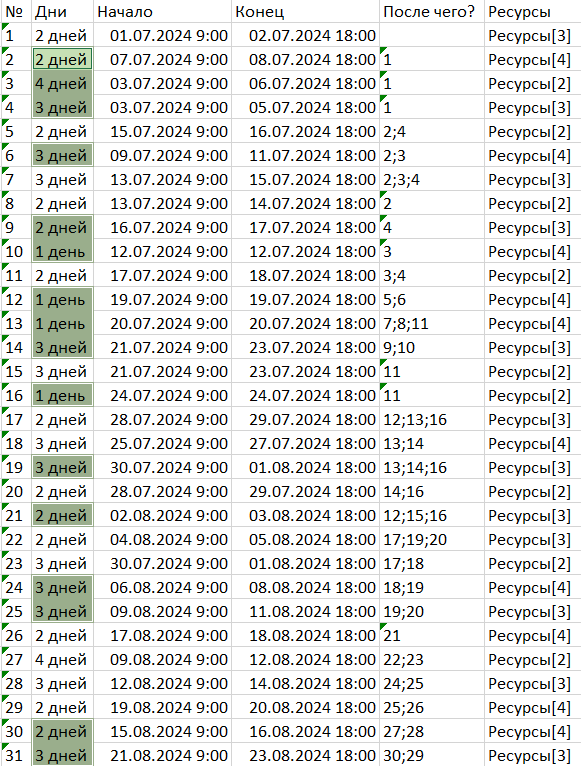
\includegraphics[height=0.6\textheight]{../img/2a2_days_change.png}\\ 
		{\LARGE Как это выглядит:}\\
		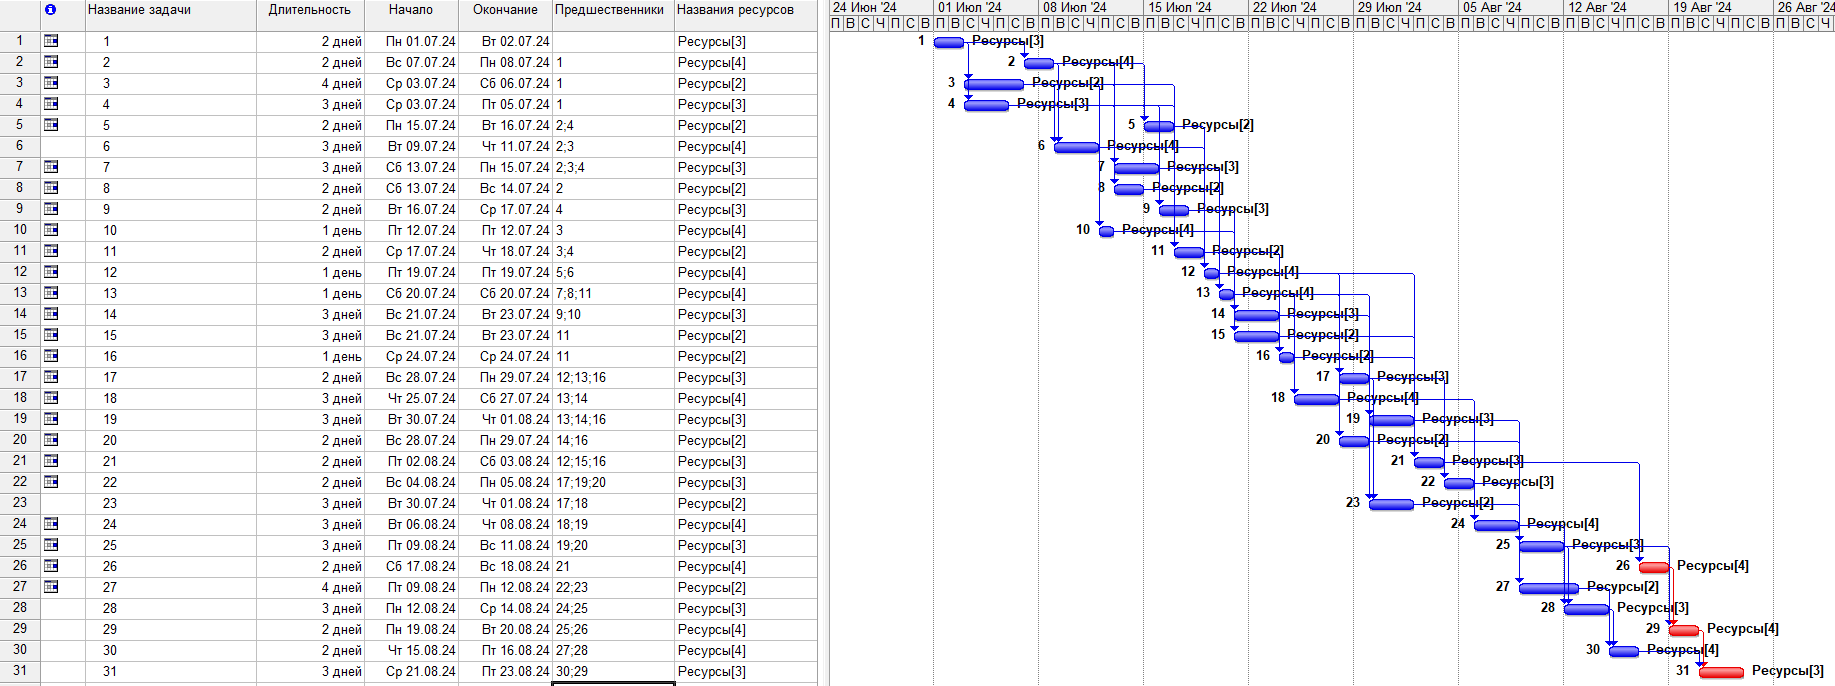
\includegraphics[width=\textwidth]{../img/ot2a2_1.png}\\
		{\LARGE Cколько оно тратит:}\\
		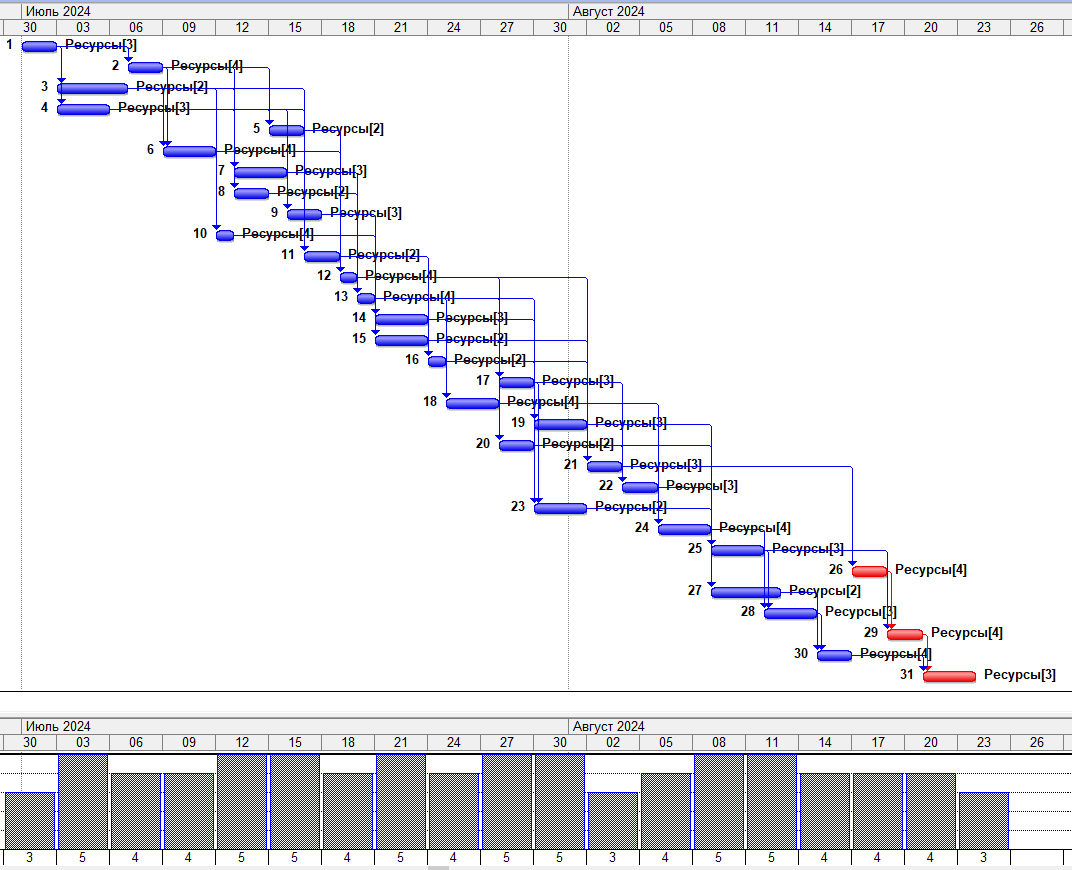
\includegraphics[width=\textwidth]{../img/2a2_answer.png}\\ 
	\subsection{Третий вариант}
		Попробуем получить ещё более лучшую дату окончания.
		В этом варианте была достигнута дата \texttt{18.08}.
		Но для достижения пришлось поменять даты по максимуму.
		Дальше эффективность улучшений сильно снижается.\\
		{\LARGE Что поменяли:}\\
		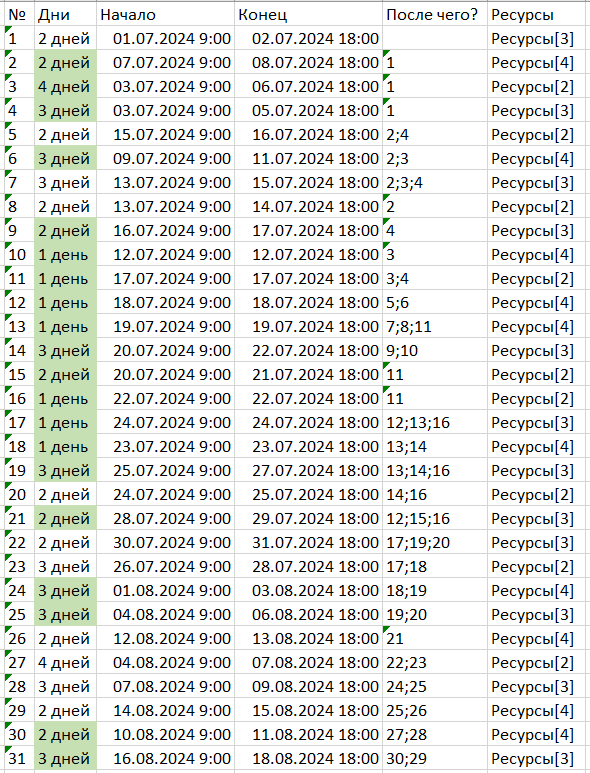
\includegraphics[height=0.6\textheight]{../img/2a3_days_change.png}\\ 
		{\LARGE Как это выглядит и сколько оно тратит:}\\
		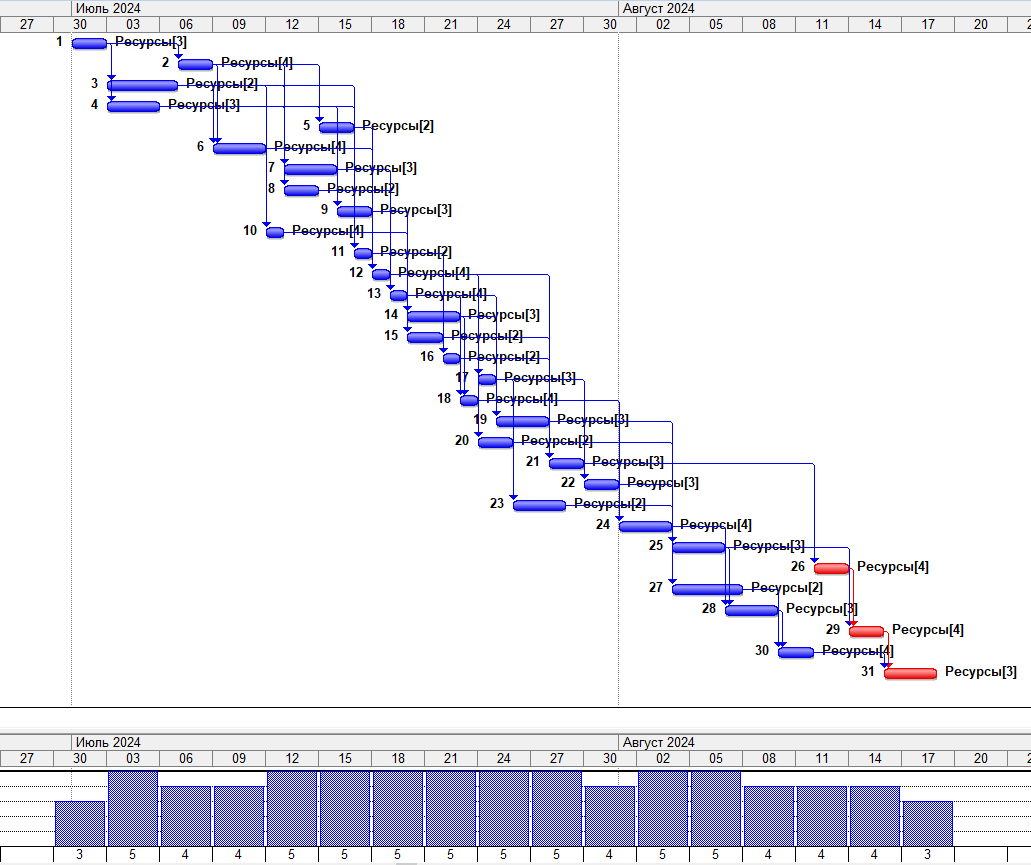
\includegraphics[width=\textwidth]{../img/2a3_answer.png}\\ 
\end{document}
